\documentclass[
	verbose,
	english,
	type=bachelor-thesis, % master-thesis
	%german,   % titles for a thesis in German, A4 paper
	paper=a4,  % forces A4 format even if <german> is not selected (useful for printing)
	%oneside,   % onesided layout
	%draft,    % omit title page, listings, and particular chapters selected below using include only
	%print,    % the printed version does not use colored links
	%final,    % removes all TODOs
]{thesis}

\addbibresource{literature/literature.bib}

% provide addon listings support:
\ThesisInternal{listings}
\LoadLanguage{R}

\ThesisInternal{pseudocode}

% do you have a glossary?
\loadglsentries{segments/glossary.tex}
% do you want colored glossary symbols in the document?
\def\glssym#1{{\color{purple!80!blue}\gls{#1}}}

\title{My Great Thesis with a Reaaaaally Reaaaaally Reaaaaally Long Title}
\author{Your Amazing Name}

\titleimage[width=.15\linewidth]{img/title-banner-image}
\date{\today}

\advisor{Prof. Dr. Matthias Tichy}{Institute of Software Engineering and Programming Languages}
% \advisor{Your Second Examiner}{Their Institute}
\supervisor{Florian Sihler}{Institute of Software Engineering and Programming Languages}

\begin{document}
\hideindraft{
	\frontmatter
		\maketitle
	
		\def\abstractblk#1{\strut\quad\sidenote{\textsc{#1}}\ignorespaces}
\begin{abstract}
   Text is funny!

   \abstractblk{Context} 

   \abstractblk{Objective}

   \abstractblk{Method} 

   \abstractblk{Limitations} 

   \abstractblk{Results} 

\end{abstract}

		\begin{acknowledgements}
   Thanksies!
\end{acknowledgements}

	
		\tableofcontents
		\listoffigures
		\listoftables
	}
	
	\mainmatter
	\setchaptertoc
\chapter{Introduction}\label{chp:introduction}
\csummary{What is the problem solved by this thesis?\csumnext What are our research questions?\csumnext What are our contributions?}

\section{Motivation}

Sample cite~\cite{DBLP:conf/msr/SihlerPSTDD24}

\begin{minted}{R}
x <- list(i='hey', j='there')
for(i in x) {
   print(paste("x$i", x$i))
}
print(x)
\end{minted}


To interpret the program above, we take \bR{x <- 2} to the set of \gls{not:N}, \gls{not:Z}, and \gls{not:R} because they describe funny numbers that we can use to index what we call an \gls{ast} (if you want the long form use \texttt{\textbackslash glsac}: \glsac{ast}). Now we can use a \gls{cpo} or verify the \gls{def:behavioral-equivalence} when interpreting the code as a \gls{formal:model}.
\gls{not:N} will not be repeated on this page!

Using the \texttt{\textbackslash glssym} macro defined in the preamble you can even color symbol uses such as \glssym{not:N} automatically if this is to your liking:
\begin{align}
   \glssym{not:N} &= \{1, 2, \ldots\} \\
   \glssym{not:Z} &= \glssym{not:N} \cup \{0\} \cup \{-1, -2, \ldots\} \\
   \glssym{not:R} &= \textit{Set of real numbers} \\
   \glssym{not:C} &= \textit{Set of complex numbers} \\
   \glssym{not:N} &\subset \glssym{not:Z} \subset \glssym{not:R} % \subset \glssym{not:C}
\end{align}

However, as you may see, \glssym{not:C} is not shown in the sidebar even though it appears first within the math mode. The reason(s) for this are manifold but in short we avoided this as math mode may be rendered multiple times. 
You can use \texttt{\textbackslash showsymbols} to propose a list of symbols to show before the math environment (using \texttt{\textbackslash showsymbols*} these will be forced as showcased below):
\begin{align}
   \showsymbols*{not:N,not:Z,not:R,not:C}
   \glssym{not:N} &= \{1, 2, \ldots\} \\
   \glssym{not:Z} &= \glssym{not:N} \cup \{0\} \cup \{-1, -2, \ldots\} \\
   \glssym{not:R} &= \textit{Set of real numbers} \\
   \glssym{not:C} &= \textit{Set of complex numbers} \\
   \glssym{not:N} &\subset \glssym{not:Z} \subset \glssym{not:R} % \subset \glssym{not:C}
\end{align}

\clearpage
\begin{figure}
   \begin{subfigure}[c]{0.33\linewidth}
      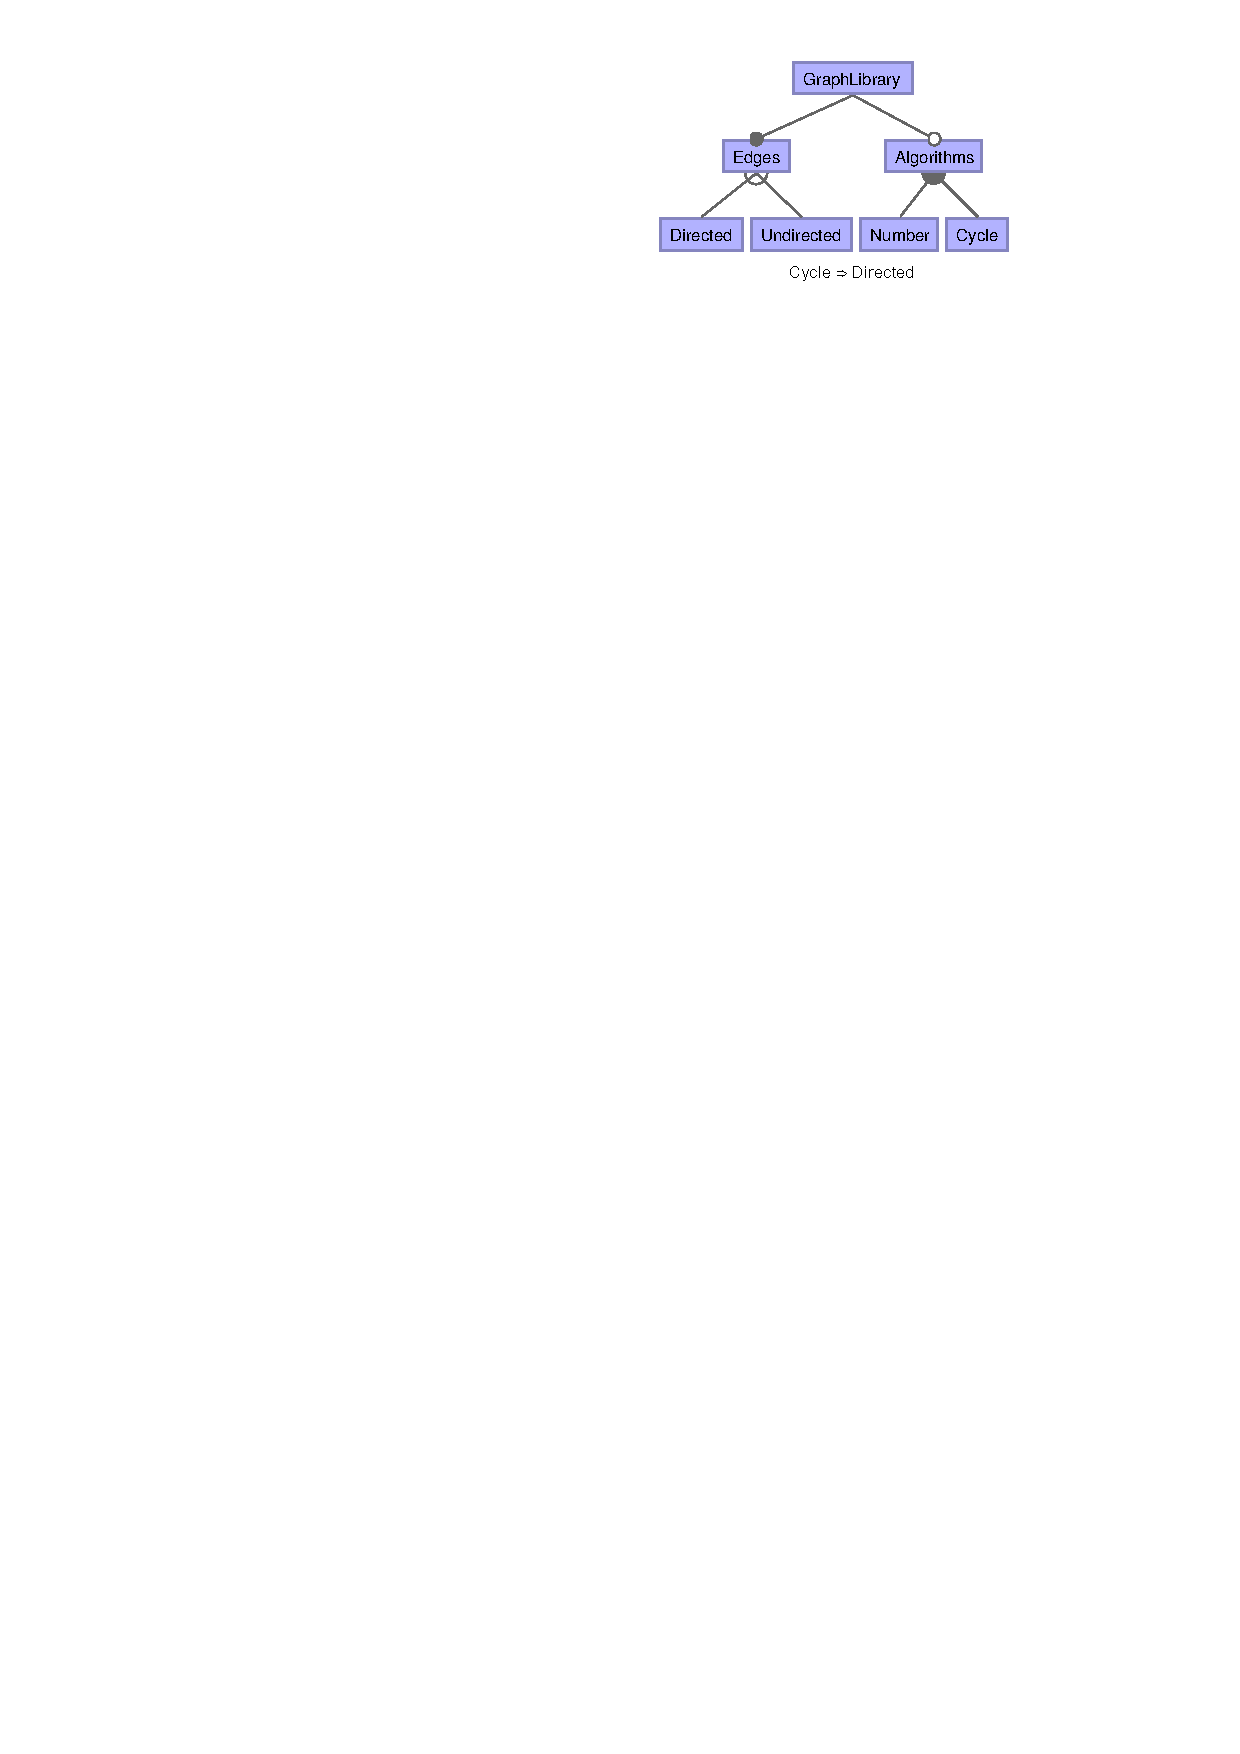
\includegraphics[width=\linewidth]{img/example.pdf}
      \caption{First subfigure.}
      \label{fig:first}
  \end{subfigure}\hfill
  \begin{subfigure}[c]{0.33\linewidth}
      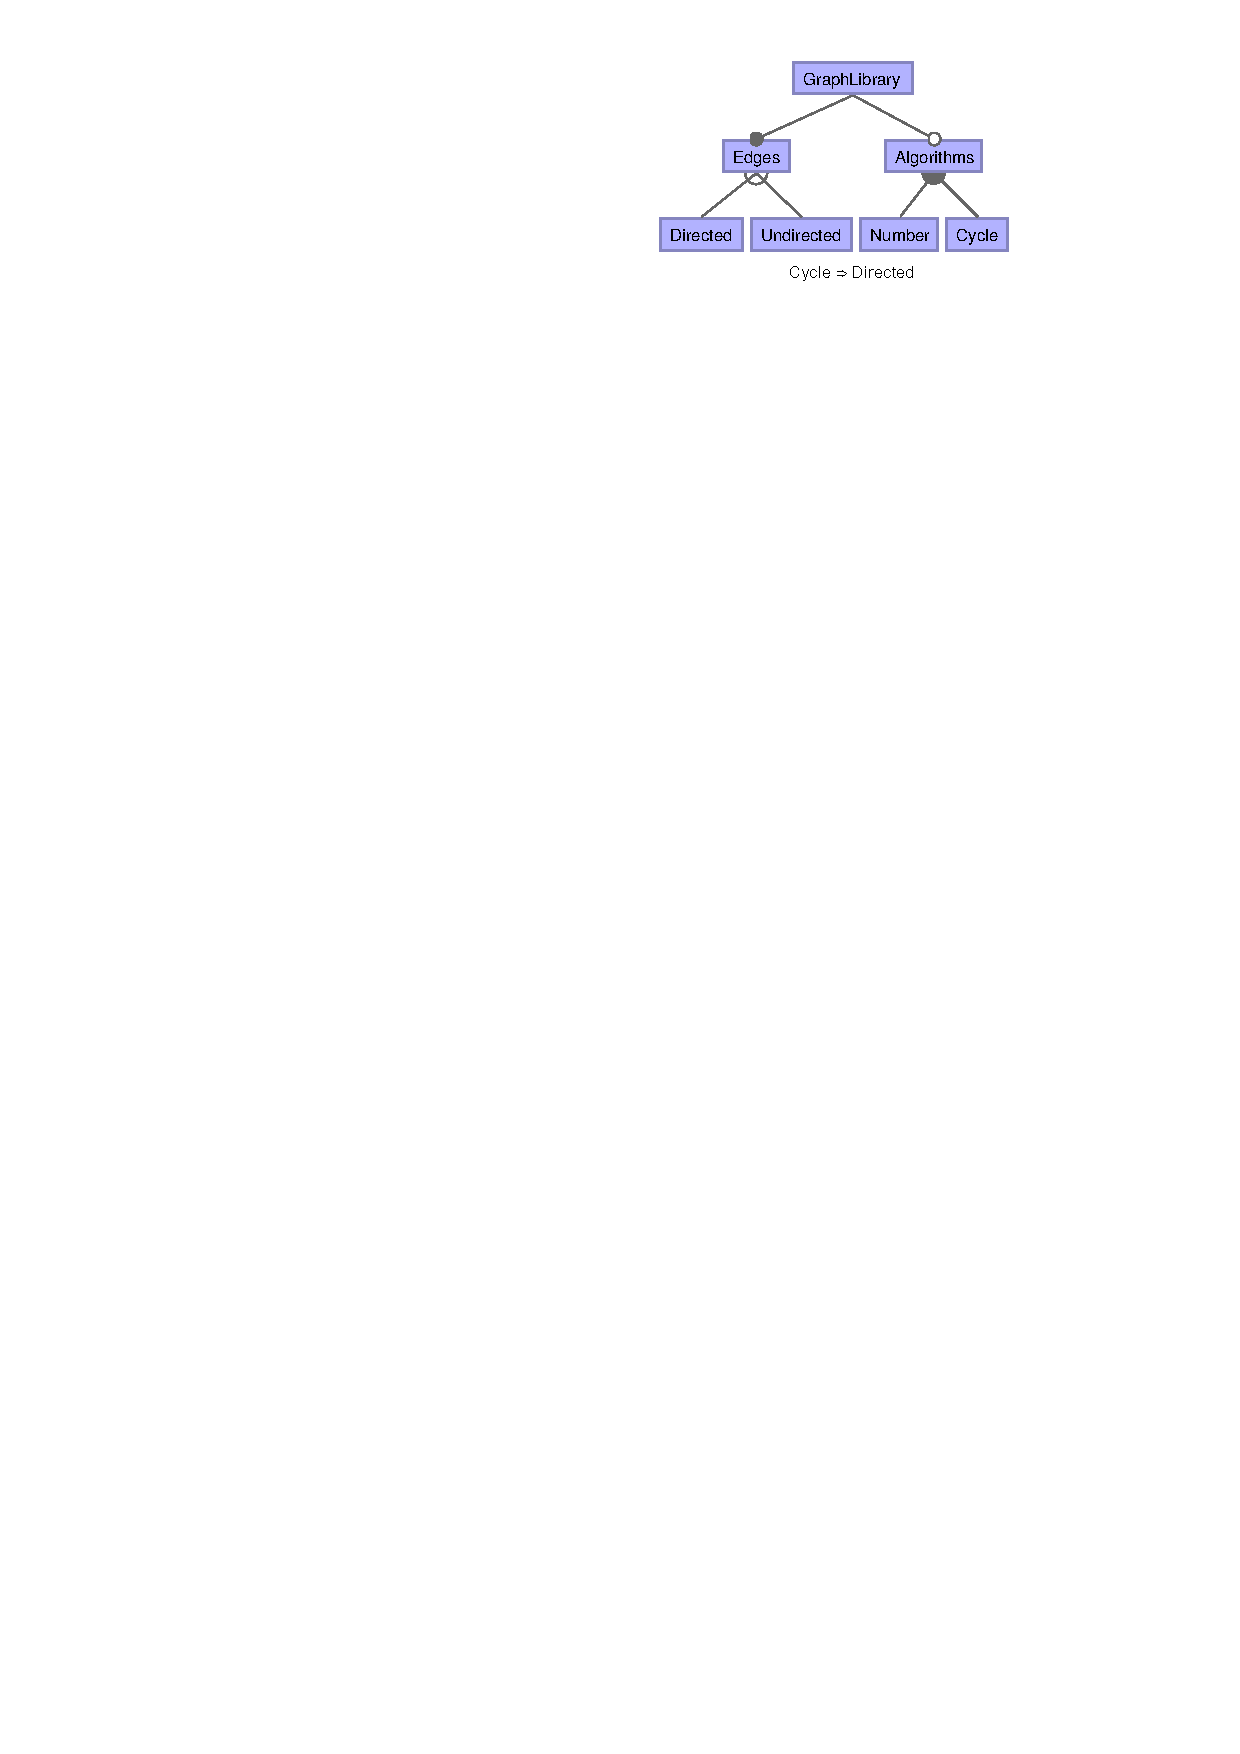
\includegraphics[width=\linewidth]{img/example.pdf}
      \caption{Second subfigure.}
   \end{subfigure}
   \caption[Main]{Main caption.}
   \label{fig:main}
\end{figure}

A viable way to group different figures is the \textit{subfigures} command, a short example can be seen at \cref{fig:main}.
This is \cref{fig:main} with the name \nameref{fig:main}.\footurl{www.google.com}{2024-12-24}
See ulm university\foothref{https://web.archive.org/web/20241221140233/https://www.uni-ulm.de/}{https://www.uni-ulm.de/}{2024-12-21} for more information.

\begin{table}
   \caption{A simple table}
   \begin{tabular}{cc}
      \toprule
      A & B \\
      \midrule
      1 & 2 \\
      3 & 4 \\
      \bottomrule
   \end{tabular}
   \label{tab:simple}
\end{table}

\section{Problem Statement}

\begin{pseudo}[tbp]
	\caption{Algo Good}
	\label{fun:good-algo}
	\begin{algorithm}[H]
		\PreCode
		\Input{x :: String}
      \Output{y :: String}
		\Output{z :: String}
		
		\StartCode
		\lIf{x \KwIs "hello"}{
         \label{alg:important-line}\Return{"world"}
      }
      \While{true}{
         \If{y \KwIs "world"}{
            \Return{"hello"}
         }
      }
      \Return{"goodbye"}
	\end{algorithm}
\end{pseudo}

In the \nameref{fun:good-algo} algorithm \cref{fun:good-algo}, an important line is \AlgoLineRef{alg:important-line}.

\begin{rqs}
   \item \label{rq:concept} What is the concept of this thesis?
   \item \label{rq:implementation} How is the concept implemented?
   \item \label{rq:evaluation} How is the implementation evaluated?
   \begin{rqs}
      \item \label{rq:evaluation:correctness} How is the correctness evaluated? \begin{rqs}
         \item Please do not nest the questions that deep!
      \end{rqs}
      \item \label{rq:evaluation:performance} How is the performance evaluated?
   \end{rqs}
\end{rqs}

We can now reference \ref{rq:concept} or with cleveref: \cref{rq:concept}.

\section{Contributions}

\section{Overview}
	\setchaptertoc
\chapter{Related Work}\label{chp:related-work}
\begin{summary}
   All the important related work!
\end{summary}

\chapter{Background}\label{chp:background}

\begin{summary}
Use this chapter only if parts of your topic are foreign in a way so that the average computer science reader needs to be introduced to it. 
\end{summary}


	\setchaptertoc
\chapter{Concept}\label{chp:concept}
\csummary{Why even concepts?\csumnext Why even A?}

\begin{summary}
The concept is\ldots
\end{summary}

\section{Formalizing Penguins}

\section{Penguin Composition}
	\setchaptertoc
\chapter{Implementation}\label{chp:implementation}
\csummary{What did change?}

\begin{summary}
Doing something completely different\ldots
\end{summary}

\section[Fun]{Petting Penguins}

\section[Happy]{How Cute Are Penguins PLS?!}

	\setchaptertoc
\chapter{Evaluation}\label{chp:evaluation}
\csummary{Is it good?}

\begin{summary}
We did\ldots
\end{summary}

\section{Methodology}

\section[Study 1]{Study 1: Penguins in the Wild}

\section[Study 2]{Study 2: Penguins in Captivity}

\section{Discussion}

\section[Threats]{Threats to Validity}
	\setchaptertoc
\chapter{Conclusion}\label{chp:conclusion}
\csummary{What is left to do, and what can be learned?}
\begin{summary}
   Within this chapter, we summarize the work of \ldots
\end{summary}

\section{Retrospective}

\section{Future Work}
	
	hello world\footnote{\the\marginparwidth Hello dello wello rello schello duello quell o} %\the\marginparwidth\marginpar{Hello dello wello rello schello duello quell o}

	\cite{DBLP:conf/msr/SihlerPSTDD24}

	\backmatter
	\printbibliography

	\let\clearpage\newpage
	\let\cleardoublepage\newpage
	\chapter{Glossary and Acronyms}
	\printglossaries

	% specify \signature{path/to/signature.png} to include a signature
	% you can also shift the signature with \signature[xshift=0pt,yshift=0pt]{path/to/signature.png}
	% if you want to set the location of the signature, use
	\signaturelocation{Ulm}
	% if you want to set the submission date of the declaration, use
	\signaturedate{2025-12-30}
	\makedeclarationofauthenticity % for a predefined declaration of authenticity
	% \begin{declarationofauthenticity} % when you want to write your own text
	% 	No, I definitely did not copy all my code from StackOverflow. I swear!
	% \end{declarationofauthenticity}
\end{document}
